\documentclass[]{book}
\usepackage{lmodern}
\usepackage{amssymb,amsmath}
\usepackage{ifxetex,ifluatex}
\usepackage{fixltx2e} % provides \textsubscript
\ifnum 0\ifxetex 1\fi\ifluatex 1\fi=0 % if pdftex
  \usepackage[T1]{fontenc}
  \usepackage[utf8]{inputenc}
\else % if luatex or xelatex
  \ifxetex
    \usepackage{mathspec}
  \else
    \usepackage{fontspec}
  \fi
  \defaultfontfeatures{Ligatures=TeX,Scale=MatchLowercase}
\fi
% use upquote if available, for straight quotes in verbatim environments
\IfFileExists{upquote.sty}{\usepackage{upquote}}{}
% use microtype if available
\IfFileExists{microtype.sty}{%
\usepackage{microtype}
\UseMicrotypeSet[protrusion]{basicmath} % disable protrusion for tt fonts
}{}
\usepackage[margin=1in]{geometry}
\usepackage{hyperref}
\hypersetup{unicode=true,
            pdftitle={Mastering R Markdown},
            pdfauthor={Michael Harper},
            pdfborder={0 0 0},
            breaklinks=true}
\urlstyle{same}  % don't use monospace font for urls
\usepackage{natbib}
\bibliographystyle{apalike}
\usepackage{color}
\usepackage{fancyvrb}
\newcommand{\VerbBar}{|}
\newcommand{\VERB}{\Verb[commandchars=\\\{\}]}
\DefineVerbatimEnvironment{Highlighting}{Verbatim}{commandchars=\\\{\}}
% Add ',fontsize=\small' for more characters per line
\usepackage{framed}
\definecolor{shadecolor}{RGB}{248,248,248}
\newenvironment{Shaded}{\begin{snugshade}}{\end{snugshade}}
\newcommand{\KeywordTok}[1]{\textcolor[rgb]{0.13,0.29,0.53}{\textbf{#1}}}
\newcommand{\DataTypeTok}[1]{\textcolor[rgb]{0.13,0.29,0.53}{#1}}
\newcommand{\DecValTok}[1]{\textcolor[rgb]{0.00,0.00,0.81}{#1}}
\newcommand{\BaseNTok}[1]{\textcolor[rgb]{0.00,0.00,0.81}{#1}}
\newcommand{\FloatTok}[1]{\textcolor[rgb]{0.00,0.00,0.81}{#1}}
\newcommand{\ConstantTok}[1]{\textcolor[rgb]{0.00,0.00,0.00}{#1}}
\newcommand{\CharTok}[1]{\textcolor[rgb]{0.31,0.60,0.02}{#1}}
\newcommand{\SpecialCharTok}[1]{\textcolor[rgb]{0.00,0.00,0.00}{#1}}
\newcommand{\StringTok}[1]{\textcolor[rgb]{0.31,0.60,0.02}{#1}}
\newcommand{\VerbatimStringTok}[1]{\textcolor[rgb]{0.31,0.60,0.02}{#1}}
\newcommand{\SpecialStringTok}[1]{\textcolor[rgb]{0.31,0.60,0.02}{#1}}
\newcommand{\ImportTok}[1]{#1}
\newcommand{\CommentTok}[1]{\textcolor[rgb]{0.56,0.35,0.01}{\textit{#1}}}
\newcommand{\DocumentationTok}[1]{\textcolor[rgb]{0.56,0.35,0.01}{\textbf{\textit{#1}}}}
\newcommand{\AnnotationTok}[1]{\textcolor[rgb]{0.56,0.35,0.01}{\textbf{\textit{#1}}}}
\newcommand{\CommentVarTok}[1]{\textcolor[rgb]{0.56,0.35,0.01}{\textbf{\textit{#1}}}}
\newcommand{\OtherTok}[1]{\textcolor[rgb]{0.56,0.35,0.01}{#1}}
\newcommand{\FunctionTok}[1]{\textcolor[rgb]{0.00,0.00,0.00}{#1}}
\newcommand{\VariableTok}[1]{\textcolor[rgb]{0.00,0.00,0.00}{#1}}
\newcommand{\ControlFlowTok}[1]{\textcolor[rgb]{0.13,0.29,0.53}{\textbf{#1}}}
\newcommand{\OperatorTok}[1]{\textcolor[rgb]{0.81,0.36,0.00}{\textbf{#1}}}
\newcommand{\BuiltInTok}[1]{#1}
\newcommand{\ExtensionTok}[1]{#1}
\newcommand{\PreprocessorTok}[1]{\textcolor[rgb]{0.56,0.35,0.01}{\textit{#1}}}
\newcommand{\AttributeTok}[1]{\textcolor[rgb]{0.77,0.63,0.00}{#1}}
\newcommand{\RegionMarkerTok}[1]{#1}
\newcommand{\InformationTok}[1]{\textcolor[rgb]{0.56,0.35,0.01}{\textbf{\textit{#1}}}}
\newcommand{\WarningTok}[1]{\textcolor[rgb]{0.56,0.35,0.01}{\textbf{\textit{#1}}}}
\newcommand{\AlertTok}[1]{\textcolor[rgb]{0.94,0.16,0.16}{#1}}
\newcommand{\ErrorTok}[1]{\textcolor[rgb]{0.64,0.00,0.00}{\textbf{#1}}}
\newcommand{\NormalTok}[1]{#1}
\usepackage{longtable,booktabs}
\usepackage{graphicx,grffile}
\makeatletter
\def\maxwidth{\ifdim\Gin@nat@width>\linewidth\linewidth\else\Gin@nat@width\fi}
\def\maxheight{\ifdim\Gin@nat@height>\textheight\textheight\else\Gin@nat@height\fi}
\makeatother
% Scale images if necessary, so that they will not overflow the page
% margins by default, and it is still possible to overwrite the defaults
% using explicit options in \includegraphics[width, height, ...]{}
\setkeys{Gin}{width=\maxwidth,height=\maxheight,keepaspectratio}
\IfFileExists{parskip.sty}{%
\usepackage{parskip}
}{% else
\setlength{\parindent}{0pt}
\setlength{\parskip}{6pt plus 2pt minus 1pt}
}
\setlength{\emergencystretch}{3em}  % prevent overfull lines
\providecommand{\tightlist}{%
  \setlength{\itemsep}{0pt}\setlength{\parskip}{0pt}}
\setcounter{secnumdepth}{5}
% Redefines (sub)paragraphs to behave more like sections
\ifx\paragraph\undefined\else
\let\oldparagraph\paragraph
\renewcommand{\paragraph}[1]{\oldparagraph{#1}\mbox{}}
\fi
\ifx\subparagraph\undefined\else
\let\oldsubparagraph\subparagraph
\renewcommand{\subparagraph}[1]{\oldsubparagraph{#1}\mbox{}}
\fi

%%% Use protect on footnotes to avoid problems with footnotes in titles
\let\rmarkdownfootnote\footnote%
\def\footnote{\protect\rmarkdownfootnote}

%%% Change title format to be more compact
\usepackage{titling}

% Create subtitle command for use in maketitle
\newcommand{\subtitle}[1]{
  \posttitle{
    \begin{center}\large#1\end{center}
    }
}

\setlength{\droptitle}{-2em}
  \title{Mastering R Markdown}
  \pretitle{\vspace{\droptitle}\centering\huge}
  \posttitle{\par}
  \author{Michael Harper}
  \preauthor{\centering\large\emph}
  \postauthor{\par}
  \predate{\centering\large\emph}
  \postdate{\par}
  \date{2018-04-30}

\usepackage{booktabs}

\usepackage{amsthm}
\newtheorem{theorem}{Theorem}[chapter]
\newtheorem{lemma}{Lemma}[chapter]
\newtheorem{corollary}{Corollary}[chapter]
\newtheorem{proposition}{Proposition}[chapter]
\newtheorem{conjecture}{Conjecture}[chapter]
\theoremstyle{definition}
\newtheorem{definition}{Definition}[chapter]
\theoremstyle{definition}
\newtheorem{example}{Example}[chapter]
\theoremstyle{definition}
\newtheorem{exercise}{Exercise}[chapter]
\theoremstyle{remark}
\newtheorem*{remark}{Remark}
\newtheorem*{solution}{Solution}
\begin{document}
\maketitle

{
\setcounter{tocdepth}{1}
\tableofcontents
}
\chapter{About the book}\label{about-the-book}

\begin{quote}
This book is in a very early stage of development. If you have any
suggestions on what should be included within this book, please get in
touch via GitHub:
\url{https://github.com/mikey-harper/mastering-rmarkdown}
\end{quote}

\begin{itemize}
\tightlist
\item
  This book aims to bring together lots of useful tips for R Markdown.
\item
  One of the common criticisms of markdown as a language is that it
  naturally limits what you can write. Users often therefore feel
  limited in what they can achieve with advanced customisation. However,
  we can easily edit.
\end{itemize}

\section{Recommended Reading}\label{recommended-reading}

There are already several fantastic books out there which you may have
already read:

\begin{itemize}
\tightlist
\item
  Dynamic documents and knitr
\item
  R Markdown: The Definitive guide
\item
  Authoring books with bookdown
\item
  Blogdown
\end{itemize}

\chapter{Introduction}\label{intro}

\begin{itemize}
\tightlist
\item
  Motivation for book
\item
  What readers can learn
\item
  Feedback and errata
\item
  Suggested examples
\end{itemize}

\section{Overview of Book}\label{overview-of-book}

\begin{itemize}
\tightlist
\item
  Explain the structure of the book
\end{itemize}

\chapter{Basics}\label{basics}

\begin{itemize}
\tightlist
\item
  What should be known before reading this book
\item
  Recommended reading
\item
  \texttt{bookdown} is used as the default engine as it provides
  improvements
\end{itemize}

\chapter{Managing Big Projects}\label{managing-big-projects}

\begin{itemize}
\tightlist
\item
  Practical tips on how a big project should be managed
\item
  \texttt{source} is particularly useful for loading external scripts so
  that the R Markdown project isn't too bloated with code.
\end{itemize}

\textbf{Ideas}: - Use \texttt{(ref:tag)} to store page formatting
options which might need to be reused. For example a page break

\section{Sourcing Files}\label{sourcing-files}

A benefit of using R Markdown is that it is easy

\begin{verbatim}
source("yourScript.R")
\end{verbatim}

\section{Caching}\label{caching}

\begin{itemize}
\tightlist
\item
  Caching
\item
  Ways it can be tailored to suit analysis. This cache invalidation is a
  great example:
  \url{https://stackoverflow.com/questions/18376008/invalidate-a-chunks-cache-when-uncached-chunk-changes}
\end{itemize}

\section{Notifications}\label{notifications}

\begin{itemize}
\tightlist
\item
  Can link R Markdown with notifications if have long analysis
\end{itemize}

\chapter{LaTeX}\label{latex}

For many authors, the main of long reports or books, the primary output
will be LaTeX. In this chapter, we discuss approaches which can be used
to customise the output of PDF reports.

Users should approach with a note of caution. One of the major benefits
of R Markdown is

\section{Inserting Commands}\label{inserting-commands}

\section{LaTeX preamble}\label{latex-preamble}

\section{Multi-figure plots}\label{multi-figure-plots}

If we need to print multiple output graphs or figures, there are several
ways this can be achieved.

\section{Cross-output}\label{cross-output}

As explained in
\url{https://bookdown.org/yihui/rmarkdown/r-code.html\#figures} of
\citet{xie2018}, we can place multiple figures side-by-side using the
\texttt{fig.hold=\textquotesingle{}hold\textquotesingle{}} along with
the \texttt{out.width} option. As an example below, we have set the
\texttt{out.width="50\%"}:

\begin{Shaded}
\begin{Highlighting}[]
\KeywordTok{plot}\NormalTok{(}\DecValTok{1}\OperatorTok{:}\DecValTok{10}\NormalTok{)}
\KeywordTok{plot}\NormalTok{(}\KeywordTok{rnorm}\NormalTok{(}\DecValTok{10}\NormalTok{), }\DataTypeTok{pch=}\DecValTok{19}\NormalTok{)}
\end{Highlighting}
\end{Shaded}

\begin{figure}
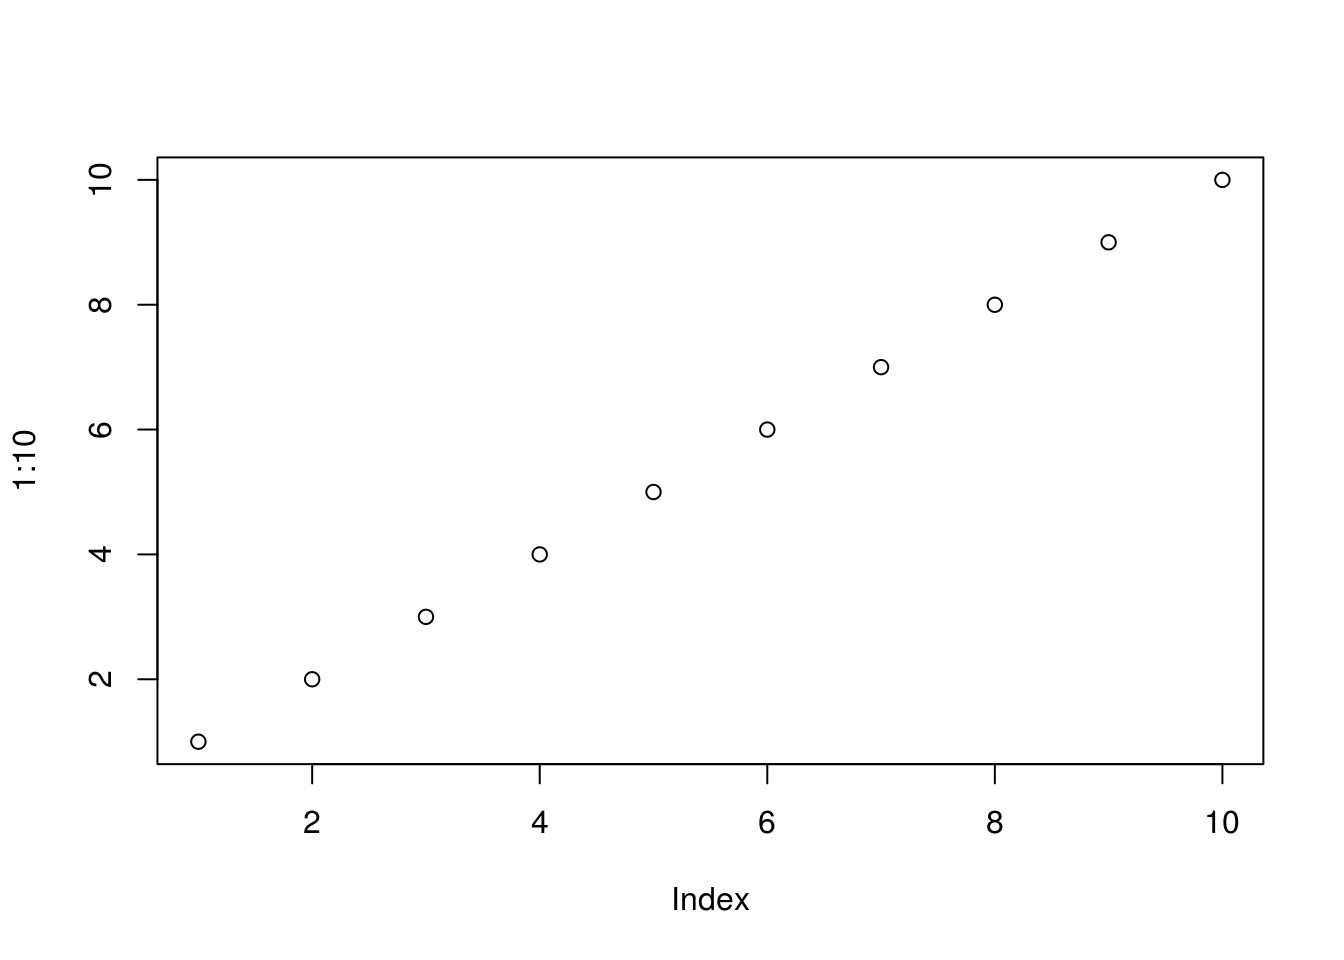
\includegraphics[width=0.5\linewidth]{mastering-rmarkdown_files/figure-latex/fig-sub-2-1} 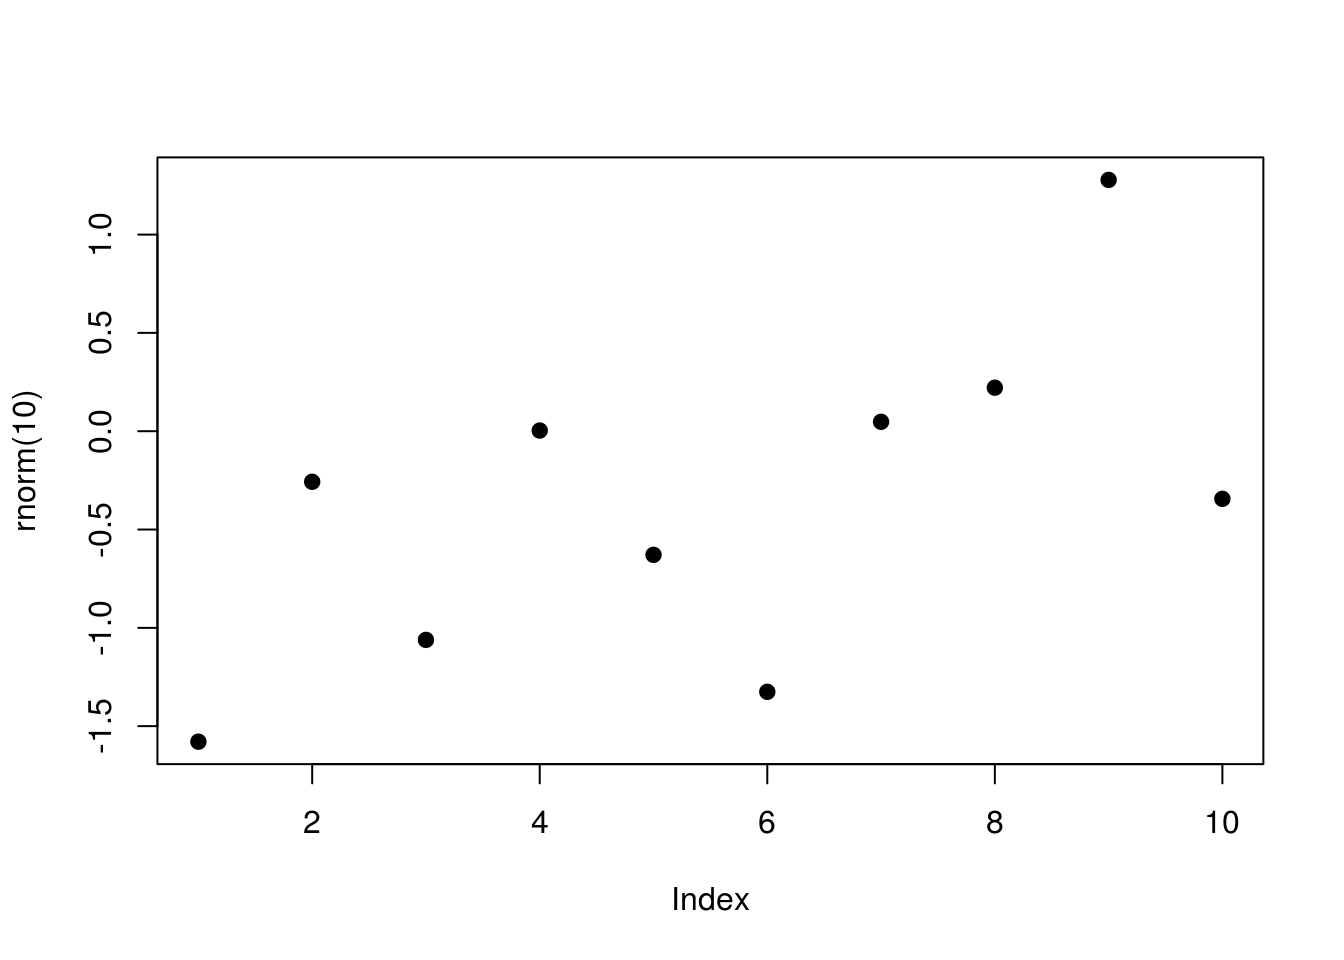
\includegraphics[width=0.5\linewidth]{mastering-rmarkdown_files/figure-latex/fig-sub-2-2} \caption{Side-by-side figures}\label{fig:fig-sub-2}
\end{figure}

The main benefits of this approach is that it is easily achieved, and
also works for both PDF and HTML outputs.

\section{LaTeX subfigures}\label{latex-subfigures}

When writing a document you may want to include some slightly more
complicated figures with multiple images. Subfigures are a useful LaTeX
feature which allows us to achieve this by plotting multiple figures
within a single plot and providing each with their own subcaption.

Subfigures require the LaTeX package \texttt{subfig}. The line
\texttt{\textbackslash{}usepackage\{subfig\}} must therefore be included
within the YAML, or if you are using an external tex template you can
add this to that file. For example:

As listed within the knitr
\href{https://yihui.name/knitr/options/}{chunk options}, subfigures
require a few additional settings to be set in the chunk header:

\begin{itemize}
\tightlist
\item
  \texttt{fig.subcap} is a list of the captions for subfigures
\item
  \texttt{fig.ncol}: the number of columns of subfigures
\item
  \texttt{out.width}: the output width of the figures. You will normally
  set this 100\% divided by the number of sub columns.
\end{itemize}

An example is demonstrated below:

\begin{verbatim}
```yaml
output: pdf_document
header-includes:
   - \usepackage{subfig}
```

```{r fig-sub, fig.cap='two plots', fig.subcap=c('one plot', 'the other one'), out.width='.49\\linewidth', fig.asp=1, fig.ncol = 2}
plot(1:10)
plot(rnorm(10), pch=19)
```
\end{verbatim}

The output is shown in Figure \ref{fig:subcaptions}.

\begin{Shaded}
\begin{Highlighting}[]
\NormalTok{knitr}\OperatorTok{::}\KeywordTok{include_graphics}\NormalTok{(}\StringTok{"images/subfigure.png"}\NormalTok{, }\DataTypeTok{dpi =} \OtherTok{NA}\NormalTok{)}
\end{Highlighting}
\end{Shaded}

\begin{figure}
\centering
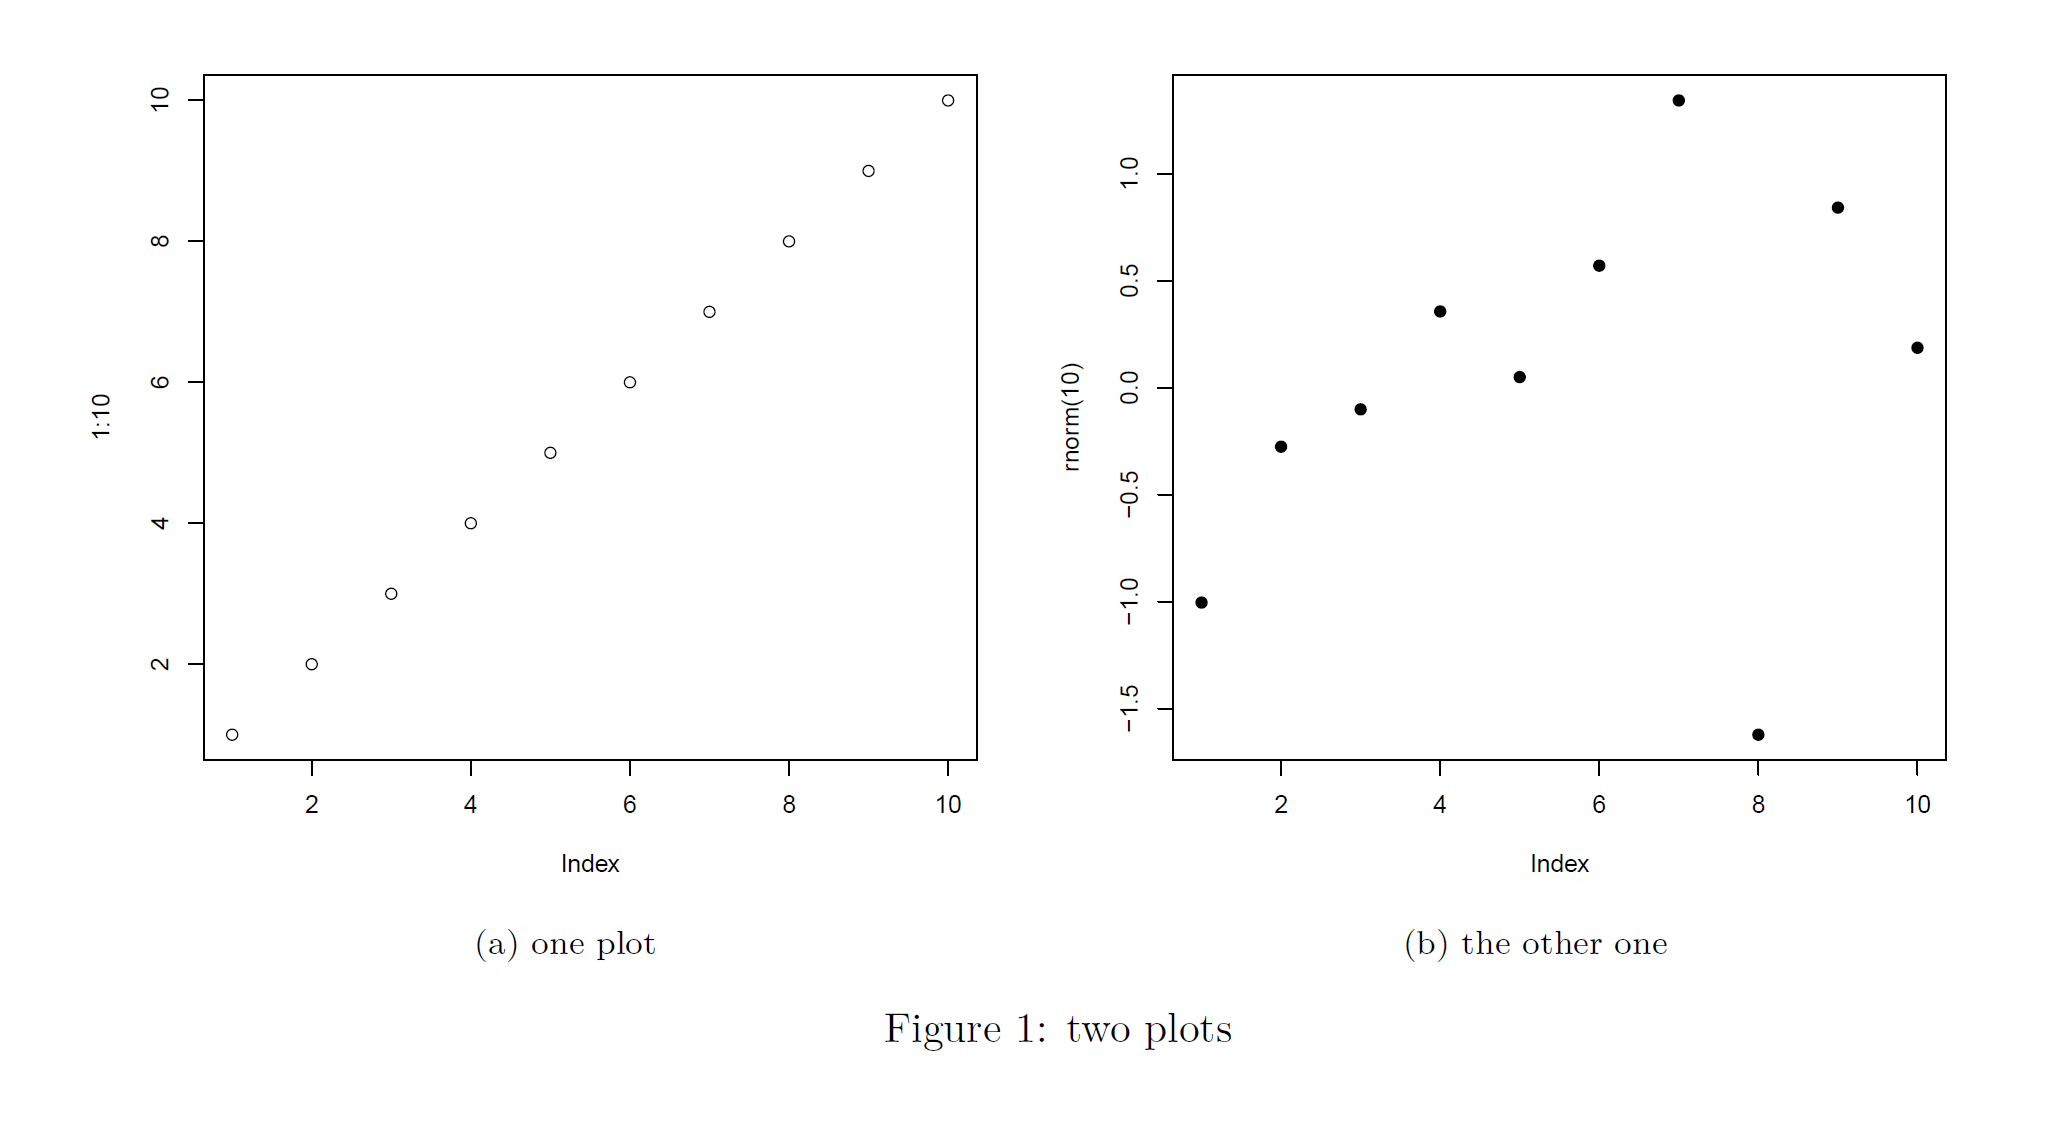
\includegraphics{images/subfigure.png}
\caption{\label{fig:subcaptions}An example subcaption}
\end{figure}

\subsection{Using with list}\label{using-with-list}

\section{Changing citation Engine}\label{changing-citation-engine}

\section{Altering Citation Style}\label{altering-citation-style}

\begin{itemize}
\tightlist
\item
  Using short author citations:
  \url{https://stackoverflow.com/questions/48303890/using-short-author-citations-in-bookdown-rmarkdown?utm_medium=organic\&utm_source=google_rich_qa\&utm_campaign=google_rich_qa}
\end{itemize}

\chapter{HTML Output}\label{html-output}

\begin{itemize}
\tightlist
\item
  Take some of the details from here:
  \url{https://rmarkdown.rstudio.com/html_document_format.html}
\end{itemize}

\section{Tabbed headings}\label{tabbed-headings}

\url{https://stackoverflow.com/questions/38062706/rmarkdown-tabbed-and-untabbed-headings?utm_medium=organic\&utm_source=google_rich_qa\&utm_campaign=google_rich_qa}

\chapter{Multi-format projects}\label{multi-format-projects}

\begin{itemize}
\tightlist
\item
  One of the main benefits of R Markdown is that it is easy to create
  documents in a single source file and generate PDF, HTML, ebook and
  Word documents. This book example is available in all three formats.
  Project should therefore ideally be designed to be flexible for the
  multiple outputs. However, users will often find themselves wanting to
  fine-tune the output, and doing so will often require -Designing
  custom behavior which can respond to change in outputs using
  \texttt{is\_latex\_output} etc. For example, you may want to have
  interactive tables using \texttt{DT:datatable} in the HTML output but
  print static versions in the PDF.
\end{itemize}

\section{Output-specific functions}\label{output-specific-functions}

\begin{itemize}
\tightlist
\item
  \textbf{bookdown} will take screenshots of HTML widgets in static
  reports
\end{itemize}

\begin{Shaded}
\begin{Highlighting}[]
\KeywordTok{library}\NormalTok{(ggplot2)}
\KeywordTok{library}\NormalTok{(plotly)}
\NormalTok{p <-}\StringTok{ }\KeywordTok{ggplot}\NormalTok{(}\DataTypeTok{data =}\NormalTok{ diamonds, }\KeywordTok{aes}\NormalTok{(}\DataTypeTok{x =}\NormalTok{ cut, }\DataTypeTok{fill =}\NormalTok{ clarity)) }\OperatorTok{+}
\StringTok{            }\KeywordTok{geom_bar}\NormalTok{(}\DataTypeTok{position =} \StringTok{"dodge"}\NormalTok{)}
\KeywordTok{ggplotly}\NormalTok{(p)}
\end{Highlighting}
\end{Shaded}

\section{Designing output}\label{designing-output}

If we wish to design our own format-specific function we can use the
functions
\texttt{knitr::is\_latex\_output()\ and}knitr::is\_html\_output`. These
function will return a TRUE/FALSE action

\begin{Shaded}
\begin{Highlighting}[]
\NormalTok{knitr}\OperatorTok{::}\KeywordTok{is_html_output}\NormalTok{()}
\end{Highlighting}
\end{Shaded}

\chapter{Knitr Hooks}\label{knitr-hooks}

\begin{itemize}
\tightlist
\item
  Knitr hooks: these are explained within previous R Markdown book
\item
  Include practical examples could be very useful for readers to see the
  power of it.
\item
  Use some of these: \url{https://gist.github.com/yihui/2629886}
\end{itemize}

\chapter{Tables}\label{tables}

\begin{itemize}
\tightlist
\item
  Using kableExtra to style tables
\end{itemize}

\chapter{References}\label{references}

\bibliography{book.bib,packages.bib}


\end{document}
